% 
% Sample latex source for a problem set
%
% Jim Teresco
% Williams College, Mount Holyoke College, Siena College
%
% Last modified: Thu Jan 27 14:56:48 EST 2011
%
% First, as you may have guessed, % is the way to define a latex 
% comment
%
% The first line tells latex you want for a default font size and that
% you want to create an ``article''
\documentclass[12pt]{article}
% extra packages to bring in
\usepackage{latexsym}
\usepackage{graphicx}      % extended graphics package
\usepackage{epsfig}        % wrapper for graphicx package
\usepackage{times}         % nicer fonts
\usepackage{url}           % better URL formatting
% set some margins, these can be defined as in, cm, pt
\setlength{\topmargin}{-0.5in}
\setlength{\textheight}{9in}
\setlength{\oddsidemargin}{0in}
\setlength{\evensidemargin}{0in}
\setlength{\textwidth}{6.5in}
\setlength{\parindent}{0in}

% a few macros that might be useful -- any time we type \eg it expands
% to the italicized version defined here
\newcommand{\etal}{{\it et al}.$\:$}
\newcommand{\eg}{{\it e}.{\it g}.$\:$}
\newcommand{\cf}{{\it cf}.$\:$}
\newcommand{\ie}{{\it i}.{\it e}.$\:$}

% This tells latex we're done defining the preamble stuff and we're
% ready to start writing the document
\begin{document}

% this removes the date that is automatically placed in the title.
% uncomment it if you want the date
%\date{}


% leave the page number off but for this page only
\thispagestyle{empty}

% For a problem set, it is not necessary to have a fancy title, so
% we just list the important information.  Note that latex will decide
% where line breaks are appropriate but we can force a line break with
% a \\ at the end of a line

Jim Teresco, Obi-Wan Kenobi, and Albus Dumbledore\\
Problem Set 0\\
Computer Science 385\\
January 11, 2011

\bigskip
\hrule
\bigskip

\noindent
1.  A simple Java program was written to copy of an array into the
arraylist.  A method called {\tt copy()} takes the value of $n$ as its
parameter, creates and fills an array of size $n$, creates an empty
{\tt ArrayList}, starts a timer, copies the values from the array to
the vector, stops the timer, and prints out the time taken.

% the verbatim environment uses our formatting and a fixed-width font -- very
% good for code snips
\begin{verbatim}
    int[] array = new int[n];
    int i;
    for (i=0; i<n; i++) array[i]=i;
	
    ArrayList v = new ArrayList(n);
    long start=System.currentTimeMillis();
    for (i=0; i<n; i++) {
        v.add(new Integer(array[i]));
    }
    long end = System.currentTimeMillis();
    System.out.println("For n="+n+", time="+(end-start));
\end{verbatim}

The following graph shows the times in milliseconds to build as {\tt
  ArrayList} from various array sizes. using the code above:

\begin{center}
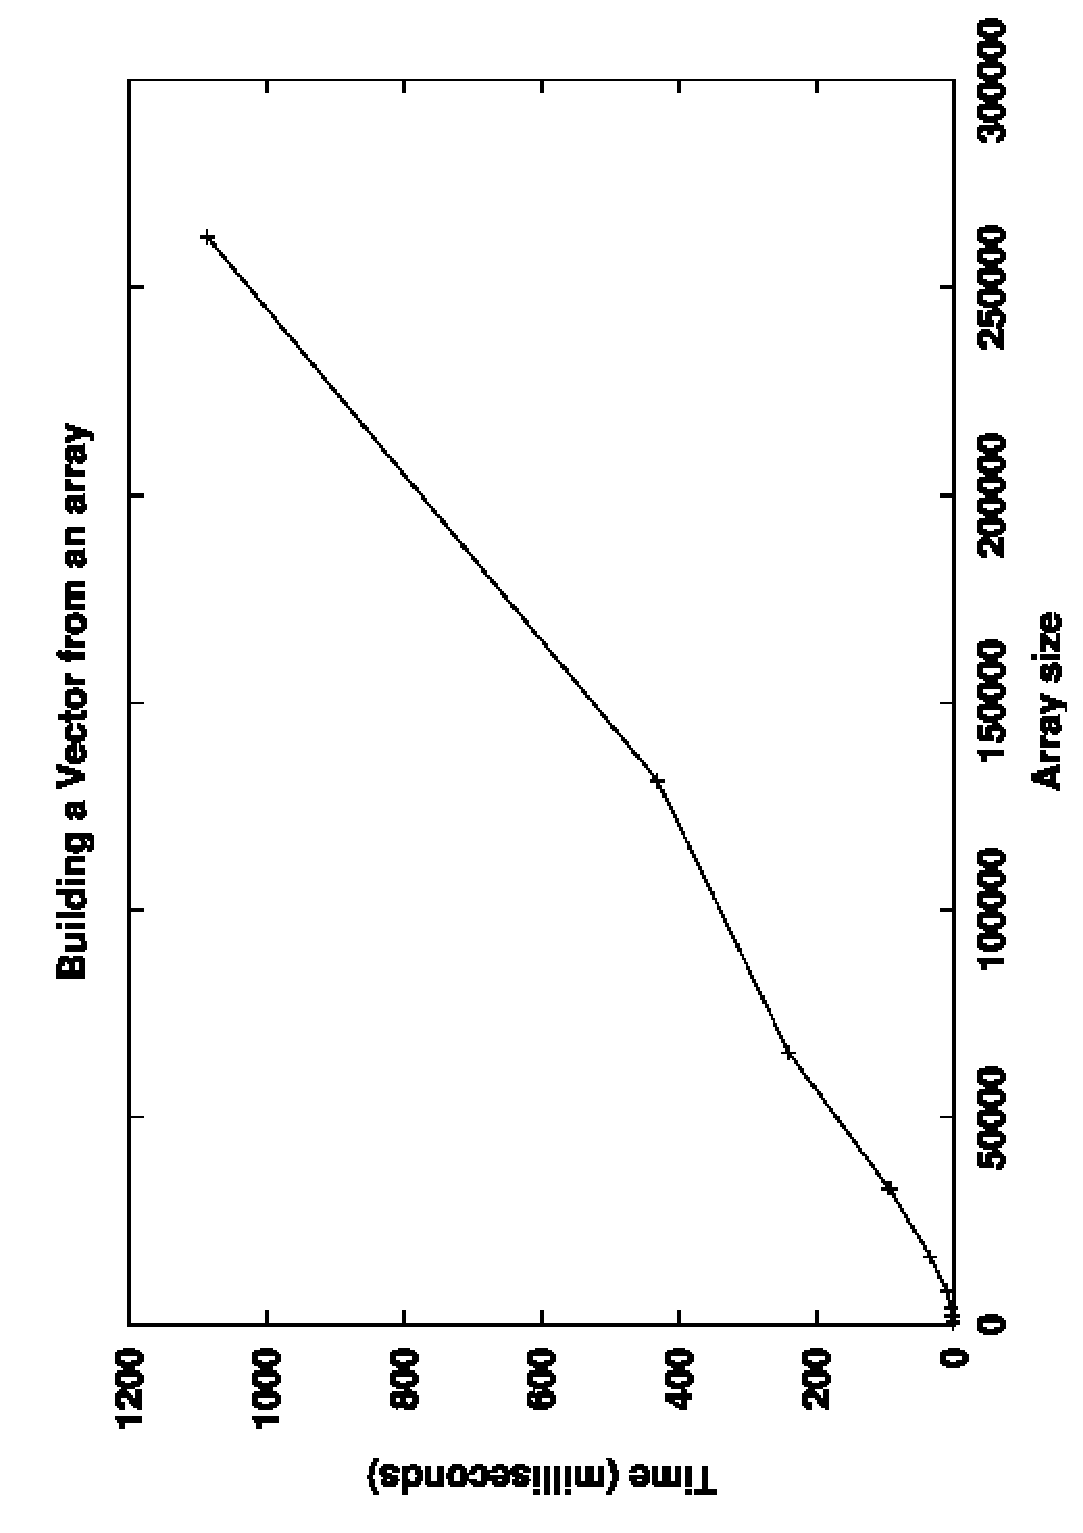
\psfig{file=times.ps,angle=-90,width=5in}
\end{center}

The method is executed 10 times for each value of $n$, and the minimum
time is taken.  The runs are all done on a PC with a 700 MHz Intel
Pentium III processor, running FreeBSD 4.3 and the Java Development
Kit version 1.3.0.  We choose array and vector sizes starting at
$n=512$ and double them until our final size $n=262,144$.  These
bounds, all powers of 2, were chosen because the 512-element case is
the first which takes at least one millisecond, and the
262,144-element is the largest which can execute without generating an
out of memory exception from the Java run-time environment.  The graph
shows the actual execution times for this method.  These times grow
linearly with the size of the array.  This agrees with the expected
$O(n)$ behavior.

\bigskip

2.  This answer involves some math mode: The equation $f(x) = x^4 +
a_0 + x^{2k}$ is nice, but how about $\frac{\alpha}{2} + \log x^y$?
Tip: see the file \url{~jteresco/shared/latexexample/isoent-ref.pdf}
for 30 pages of special characters and how to make \LaTeX{} print
them.

Here's some more math, just for fun.

\begin{enumerate}
  \item $N \in \Omega(\log N)$
  \item $5N + 6 \in \Theta(N)$
  \item $N \log N \in \Omega(N)$
  \item $N \in \Theta(N – N^{\frac12})$
\end{enumerate}

And some others.


\begin{itemize}

\item $f(n) \in O(f(n))$

\item $f(n) \in O(g(n))$ iff $g(n) \in \Omega(f(n))$

\item If $f(n) \in O(g(n))$ and $g(n) \in O(h(n))$, then $f(n) \in
  O(h(n))$

\item If $f_1(n) \in O(g_1(n))$ and $f_2(n) \in O(g_2(n))$, then
  $f_1(n) + f_2(n) \in O(\max\{g_1(n),g_2(n)\})$

\end{itemize}


We can do limits.  This equation will be larger and centered.

$$
\lim_{n\to\infty}\frac{f(n)}{g(n)}
$$

We can compute summations.

$$
\sum_{i=1}^n i = \frac{n(n-1)}{2}
$$

Next, let's work toward a more general result:
$$
an^2 + bn + d \in O(n^2)
$$
for positive constants $a$, $b$, $d$.

We proceed by noting that
$$
an^2 + bn + d \leq an^2 + bn + n
$$
for $n>d$, and
$$
an^2 + bn + n = an^2 + (b+1)n \leq an^2 + n^2
$$
for $n>b+1$, and
$$
an^2 + n^2 = (a+1)n^2
$$
which leads us to constants of $c=a+1$ and $n_0=\max(d,b+1)$.


\bigskip

3.  Parallel environments for network performance comparisons.
Variations in architecture, interprocess communication vehicles,
numbers of processes and computers are examined.

\begin{center}
\begin{tabular}{|l|l|c|c|l|}
\hline
{\bf Architecture} & {\bf IPC vehicle} & {\bf Procs.} & {\bf
Computers} & {\bf Key}
\\ \hline \hline
IBM SP2 & switch & 2--32 & 2--32 & SP2s \\ \hline
IBM SP2 & Ethernet & 2--32 & 2--32 & SP2e \\ \hline
Sun Ultra 2/2200 & shared memory & 1--2 & 1 & SUNsh \\ \hline
Sun Ultra 2/2200 & local p4 & 1--2 & 1 & SUNlp4 \\ \hline
Sun Ultra 2/2200 & Ethernet p4 & 1--6 & 1--3 & SUNp4(10) \\ \hline
Sun Ultra 2/2200 & fast Ethernet p4 & 1--6 & 1--3 & SUNp4(100) \\ \hline
SGI Onyx II & shared memory & 1--8 & 1 & SGIsh \\ \hline
SGI Onyx II & local p4 & 1--8 & 1 & SGIlp4 \\ \hline
\end{tabular}
\end{center}

\bigskip

4.  This question's answer involves bulleted lists for some reason.

\begin{itemize}

\item Item 1.

\item Item 2.

  \begin{itemize}
   \item subitem of 2!
   \item another subitem of 2.
  \end{itemize}

\end{itemize}

Maybe you want them numbered:

\begin{enumerate}

\item I bet this gets 1.

\item And this gets 2.

\end{enumerate}

\bigskip

5. How to compile your \LaTeX{} source into something readable and printable.

To compile this file into a device independent ({\tt .dvi}) file:

\begin{verbatim}
latex paper.tex
\end{verbatim}

Then convert to postscript:

\begin{verbatim}
dvips -P pdf -t letter paper.dvi -o
\end{verbatim}

You can actually leave off the ``-P pdf -t letter'' if all you want is
postscript.  Those options are there to allow conversion to a better
PDF file when you run

\begin{verbatim}
ps2pdf paper.ps
\end{verbatim}

You can view your postscript files with {\tt ghostview}, or if you
are lucky, with {\tt gv}.

% tell latex we're done.  Anything beyond this line will be ignored.
\end{document}

This doesn't show up, because it came after the \end{document}
